%% ceci est un commentaire 
%% il faut toujours commencer par \documentclass[type de papier, taille de texte]{sytle du document}
\documentclass[a4paper,10pt]{report} %%%% sytle du document : report/book/article


%%%%%%%%%%%%%%%%%%%%%%%%%%%%%%%%%%%%%%%%%%%%%%%%%%%%%%%%%%%%%%%%%%%%%%%%%%%%%%%
%% la suite est une collection des "package" ou des "librararies" pour utiliser des codes spécifiques

%% il vous suffit de les copie-coller quand vous créez un nouveau document TeX (ou bien en ajouter plus si besoin).
\usepackage[utf8]{inputenc} %% pour les accents en français
\usepackage[frenchb]{babel} %% pour un format français
\usepackage{graphicx} %% pour afficher des graphiques
\usepackage{amsmath} %% pour écrire des symboles (maths), des équations, etc.
\usepackage{amssymb}
\usepackage{color}
\usepackage{bm} %% pour lister des citations/la biblio
\usepackage{hyperref} %% pour inserer des liens internet
\usepackage{cleveref} %% pour faire des références uax équations, tableaux, etc.
%\usepackage{setspace} %% pour changer l'espace entre les lignes
%\linespread{1.6} %% pour changer l'espace entre les lignes












%%%%%%%%%%%%%%%%%%%%%%%%%%%%%%%%%%%%%%%%%%%%%%%%%%%%%%%%%%%%%%%%%%%%%%%%%%%%%%%
\title{\textbf{Modélisation d'un treillis par éléments finis BE à rendre rédigé}} %% choissez un titre approprié à votre sujet
\author{par\\ZHANG Xunjie\\pour le UE Atelier Numérique en Mécanique M1 } %% utilisez \\ pour une novuelle ligne
\date{fait le 19 avril 2017} %% pour afficher la date actuelle commenter cette ligne














%%%%%%%%%%%%%%%%%%%%%%%%%%%%%%%%%%%%%%%%%%%%%%%%%%%%%%%%%%%%%%%%%%%%%%%%%%%%%%%
%% TOUT ce qui va dans votre rapport doit être entre \begin{document} & \end{document}
\begin{document}
\selectlanguage{french} %% format français
\maketitle %% pour afficher le titre
\tableofcontents %% pour afficher/compiler le sommaire automatiquement
\listoffigures %% pour lister les figures
%%%%%%%%%%%%%%%%%%%%%%%%%%%%%%%%%%%%%%%%%%%%%%






%%%%%%%%%%%%%%%%%%%%%%%%%%%%%%%%%%%%%%%%%%%%%%
\chapter{Définition du treills à etudier}
\section{Définition}
On se propose d'étudier la modélisation d'un treillis par élément finis .Un treillis est un assemblage de poutres métaliques et on suppose que cet assemblage subit uniquement des efforts de compression (ou extension ) sans effect flextion .On peut aussi dire que cettes poutres sont barres . \\

Le treillis est constitué de poutres d'acier , on a :
\begin{itemize}
    \item[$\bullet$]$E=2\times 10^8\,Pa$
    \item[$\bullet$]$S=0.0025\,m^2$
    \item[$\bullet$]$\rho=7860\,kg/m^3$
\end{itemize}

Mon numéro d'étudiant est 11310840 , on a :
\begin{itemize}
    \item[$\bullet$]$a=0$
    \item[$\bullet$]$b=8$
    \item[$\bullet$]$c=4$
    \item[$\bullet$]$d=0$
\end{itemize}

\section{Conditions limites}
Le treillis contient 12 noeuds et on applique systèmatiquement les conditions suivantes :
\begin{itemize}
    \item[$\bullet$]encastrement au noeud 1
    \item[$\bullet$]déplacement vertical nul au noeud 4 et 6 $(c+2)$
    \item[$\bullet$]déplacement horizontal nul au noeud 9 et 10 $(b+2)$
    \item[$\bullet$]on applique une force extérieure au noeud 12 de composantes $F_x=1000N\,,F_y=1*100=100N$
     \item[$\bullet$] le chiffre $a$ donne la forme du treillis numéro $10$
\end{itemize}


\section{Ebauche du treillis}


\begin{figure}[h]
\centering
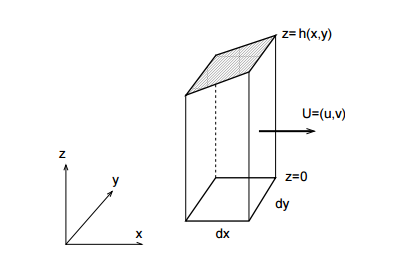
\includegraphics[width=0.8\textwidth]{fig/figure1.png}
\caption{ébauche du treillis}
\end{figure}



%%%%%%%%%%%%%%%%%%%%%%%%%%%%%%%%%%%%%%%%%%%%%%
\chapter{Etude statique du treillis}
\section{Démarche}
On analyse une poutre d'abord dans la référence local ,on utilise la méthode éléments finis et on a la matrice élémentaire , ensuite on transforme cette matrice locale à référence globale . Et on fait les mêmes mesure pour les autre poutre et on fait assemblage . Sur la programme python ,d'après on applique les conditions limites , on peut trouver la dééfomation sur chaque noeud .
\section{Déformation}
On fait une figure du treillis , dans laquelle on se trouve la déformation du treillis après on applique la force extérieure et conditions limites . 
\begin{figure}[h]
\centering
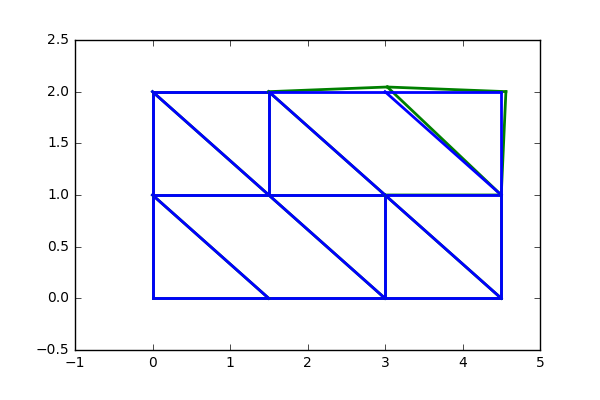
\includegraphics[width=1.0\textwidth]{fig/deforme.png}
\caption{déformation du treillis}
\end{figure}

Dans la figure , on peut voir au noeud 8 , 11 et 12 , il y a une grande déplacement , on peut dire que la poutre entre noeud 10 et 11 , la poutre entre noedu 11 et 12 sont plus sollicitées .Et les autres , il n'y pas de déplacement évident , et on se trouve aussi les déplacement sont nulles dans la ficher associée "déformation.txt"
\section{Changement de section}
Sur la programme python , on change la section du treillis ( 0.5 plus grand et plus petite) , on trouve les déformetion est proportion inverse que la section du treillis . On peut aussi avoir la même résultat dans la analyse théorique .



%%%%%%%%%%%%%%%%%%%%%%%%%%%%%%%%%%%%%%%%%%%%%%
\chapter{Etude en dynamique}
\section{Démarche et valide python}
Il est en même procédure que l'etude statique , mais cette fois , la matrice raideur élémentaire  est changée par la matrice de masse élémentaire .  Les plusations carrés sont les valeur propres de la matrice $A$ ,cequi est la product de l'inverse de matrice de masse total avec la matrice de raideur total.  

\section{Dynamique}

\begin{figure}[h]
\centering
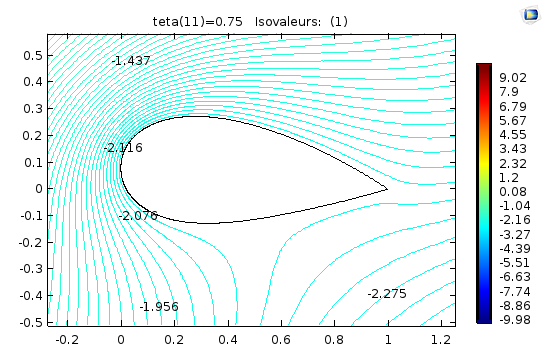
\includegraphics[width=1.0\textwidth]{fig/figure3.png}
\caption{les pulsation du treillis}
\end{figure}
 Les valeurs ci-dessus sont $\omega^2$ .


%%%%%%%%%%%%%%%%%%%%%%%%%%%%%%%%%%%%%%%%%%%%%%
\chapter{Programme Python}
Vous pouvez touver la programme Python sur moodle ou je l'ai déja déposé .%%%%%%%%%%%%%%%%%%%%%%%%%%%%%%%%%%%%%%%%%%%%%%
\chapter{Conclusion}

Dans cette séance de TP , on etude le treillis de triangle , c'est un treillis très simple mais qui nous donne une idée pour modilifier un autre treilli compliqué . 

On utilise Python pour programmer et on etude comment ouvrir et créer une file sur python .

Pour etudierun  treillis compliqué , on peut utiliser python pour connâtre les informations du treillis . on va savoir la stabilité par étude dynamique et on peut trouver les fréquence sollicités . 






\bibliography{MonBiblio.bib}
\bibliographystyle{unsrtnat}	
\end{document}
\grid
